\documentclass[10pt,xcolor=table]{beamer}

\usetheme[subsectionpage=progressbar]{metropolis}
\setbeamertemplate{itemize subitem}{--}
\setbeamerfont{caption}{size=\footnotesize}
\usepackage{appendixnumberbeamer}

\usepackage{listings}
\lstset{
  basicstyle=\footnotesize\ttfamily,
  backgroundcolor = \color{gray!20}
}
\lstdefinestyle{c}{language=C,
  keywordstyle=\bfseries\color{green!40!black},
  commentstyle=\itshape\color{purple!40!black},
  % identifierstyle=\color{blue},
  stringstyle=\color{orange}
}
\lstdefinestyle{shell}{language=sh,
  commentstyle=\itshape\color{purple!40!black},
  moredelim=**[is][\only<2->{\color{red}}]{@}{@},
  moredelim=**[is][\only<3>{\color{blue}}]{¿}{¿}
}
\lstdefinestyle{asm}{language=[x86masm]Assembler,
  commentstyle=\itshape\color{purple!40!black},
}
\lstdefinestyle{valgrind}{basicstyle=\footnotesize\ttfamily,
  backgroundcolor = {},
}
\usepackage{caption}
\captionsetup[lstlisting]{font={small,tt}, labelformat=empty,
  labelsep=none}

\usepackage{booktabs}
\usepackage[scale=2]{ccicons}

\usepackage{pgfplots}
\usepgfplotslibrary{dateplot}

\usepackage{expl3}
\ExplSyntaxOn
\int_zero_new:N \g__prg_map_int
\ExplSyntaxOff
\usepackage{tikz}
\usetikzlibrary{tikzmark,decorations.pathreplacing,calligraphy}

% Figure's path
\graphicspath{{./figs/}}

\title{Optimization and Profiling of HPC Applications}
\subtitle{using free software resources}
\date{\today}
\author{Emilio J. Padrón González}
 \institute{\href{mailto:emilioj@udc.gal}{\nolinkurl{emilioj@udc.gal}}
   -- \url{http://gac.udc.es/~emilioj}\\Computer Architecture Group
   -- Universidade da Coruña}

\begin{document}

\maketitle

\begin{frame}{Outline}
  \setbeamertemplate{section in toc}[sections numbered]
  \tableofcontents[hideallsubsections]
\end{frame}

\begin{frame}{Contents: Lesson 1}
  \setbeamertemplate{section in toc}[sections numbered]
  \setbeamertemplate{subsection in toc}[ball unnumbered]
  \tableofcontents[sections={1-2}]
\end{frame}

% \begin{frame}{Contents: Lesson 3}
%   \setbeamertemplate{section in toc}[sections numbered]
%   \setbeamertemplate{subsection in toc}[ball unnumbered]
%   \tableofcontents[sections={3}]
% \end{frame}


\section{Optimization and Profiling of Parallel Code}

\subsection{Paraver et al: an overview}

\frame{
  \frametitle{\insertsectionhead}
  % \item ompP
  \begin{block}{Leveraging BSC's HPC Performance
      Tools~\footnote{Barcelona Supercomputing Center Performance
        Tools: \url{http://tools.bsc.es}\\~~~Repositories:
        \url{http://github.com/bsc-performance-tools}} to profile and
      optimize parallel applications}
    \begin{center}
      Basic toolchain:~~~~~~~~~~~~~~~~~~~~~~~~~~~~~~~~~~~~~~~~~~~~~~~~~~~~~~~~~~~~~~~~~
    \item Extrae $\Rightarrow$ Paraver $\Rightarrow$ Dimemás
    \end{center}
  \end{block}

  \begin{description}
  \item[Extrae:] package that generates Paraver-trace files for
    a post-morten analysis
  \item[Paraver:] trace visualization and analysis browser
  \item[Dimemás:] high-abstracted network simulator for message-passing programs
  \end{description}
}

\frame{
  \frametitle{BSC's performance analysis tools}

  Let's embrace again this \underline{core idea} (from a previous slide):
  \begin{quote}
    Profile first, optimize later
  \end{quote}
  \begin{itemize}
  \item Analysis must be the first step towards the optimization of an
    application
  \item Performance analysis tools allow us to identify and
    characterize the inefficiencies that cause a poor performance
  \end{itemize}

  \pause

  \begin{block}{BSC's toolchain main objectives:}
    \begin{itemize}
    \item flexibility and versatility: platforms, environments,
      programming models\ldots
    \item simplify and facilitate the process of extracting information from the performance data
    \end{itemize}
  \end{block}
}

\frame{
  \frametitle{Extrae}

  {\bf Extrae}: dynamic instrumentation package to trace programs
  \begin{itemize}
  \item Generates trace files that can be later visualized with {\bf
      Paraver}
  \item Works with different programming models:
    \begin{itemize}
    \item shared memory model (such as OpenMP and pthreads)
    \item the message passing (MPI)
    \item hybrid
    \end{itemize}
  \end{itemize}
}

\frame{
  \frametitle{Extrae: main features}

  \begin{itemize}
  \item Parallel programming models \tikzmark{start}
    \begin{itemize}
    \item MPI, OpenMP, pthreads, OmpSs, CUDA, OpenCL,\\ Java, Python\ldots
    \end{itemize}
  \item Platforms
    \begin{itemize}
    \item Intel, Cray, BlueGene, MIC, ARM, Android,\\ Fujitsu Spark\ldots
    \end{itemize}
  \item Performance Counters
    \begin{itemize}
    \item Using PAPI interface
    \end{itemize}
  \item Link to source code
    \begin{itemize}
    \item Callstack at MPI routines
    \item OpenMP outlined routines
    \item Selected user functions (Dyninst)
    \end{itemize}
  \item Periodic sampling \tikzmark{end}
  \item User events (Extrae API)
  \end{itemize}

  \begin{tikzpicture}[remember picture,overlay]
    \draw[decorate,decoration={calligraphic brace}]
    ([yshift=10pt,xshift=150pt]{{pic cs:end}|-{pic cs:start}}) --
    node[xshift=5pt,anchor=west] {\parbox{5cm}{No need to\\ recompile/link!}}
    ([xshift=150pt]{pic cs:end})
    ;
  \end{tikzpicture}
}

\frame{
  \frametitle{Extrae: how it works}

  \begin{itemize}
  \item Symbol substitution through LD\_PRELOAD \hfill \alert{\bf $\leftarrow$ Recommended!}
    \begin{itemize}
    \item Specific \underline{tracing libraries} for each combination of runtimes
      \begin{itemize}
      \item MPI
      \item OpenMP
      \item OpenMP+MPI
      \item \ldots
      \end{itemize}
    \end{itemize}
  \item Dynamic instrumentation
    \begin{itemize}
    \item Based on DynInst (developed by U.Wisconsin/U.Maryland)
      \begin{itemize}
      \item Instrumentation in memory
      \item Binary rewriting
      \end{itemize}
    \end{itemize}
  \item Alternatives
    \begin{itemize}
    \item Static link (i.e., PMPI, Extrae API)
    \end{itemize}
  \end{itemize}
}

\frame{
  \frametitle{Extrae: typical scenario}

  \begin{itemize}
  \item Traces are obtained with {\bf Extrae} in a Supercomputer
    running the code to optimize:
    \begin{itemize}
    \item using the {\tt LD\_PRELOAD} mechanism to intercept entries and
      exits to MPI
    \item data from hardware counters (cache misses, instructions and
      cycles) at those points
    \end{itemize}
  \item Traces are analysed post-mortem in a PC with {\bf Paraver},
    and maybe also with {\bf Dimemas}
  \item Batch analysis possibility: {\bf Paramedir}
  \end{itemize}
}

\frame{
  \frametitle{Extrae: how to use it}

  In a nutshell:
  \begin{enumerate}
  \item Adapt the job submission script
  \item \structure{[optional]} Tune the Extrae XML configuration file
    \begin{itemize}
    \item~\mbox{Examples distributed with Extrae: {\footnotesize \tt
          \$EXTRAE\_HOME/share/example}~\footnote{In Finisterrae
          II:\\~~~{\scriptsize EXTRAE\_HOME=/opt/cesga/easybuild-cesga/software/MPI/gcc/6.4.0/openmpi/2.1.1/extrae/3.5.2}}}
    \end{itemize}
  \item Run the job to generate the trace
  \end{enumerate}
}

\begin{frame}[fragile]{Extrae: submission script}

  \vspace*{-0.2cm}
  \begin{lstlisting}[style=shell,gobble=3,caption={submit\_trace.sh}]
    #!/bin/sh
    #SBATCH -t 00:20:00 # execution time hh:mm:ss *OB*
    #SBATCH -n 16 #tasks (MPI processes)
    #SBATCH -c 24 #cores/task (shared-mem threads/process)
    ##SBATCH -N 16  #nodes
    #SBATCH -p cola-corta

    @module load extrae/3.5.2
    # export TRACE_NAME=trace_filename.prv # *OP*
    @
    srun -n 16 @${HOME}/trace.sh@ parallel_binary [params]
  \end{lstlisting}

  \pause

  \vspace*{-0.2cm}
  \begin{lstlisting}[style=shell,gobble=3,caption={trace.sh}]
    #!/bin/sh
    source /opt/cesga/easybuild-cesga/software/MPI/gcc/6.4.0\
                    /openmpi/2.1.1/extrae/3.5.2/etc/extrae.sh
    ¿export EXTRAE_CONFIG_FILE=${HOME}/extrae.xml¿
    ¿export LD_PRELOAD=${EXTRAE_HOME}/lib/libmpitrace.so¿ # C code

    $*     # Run the program
  \end{lstlisting}
\end{frame}

\frame{
  \frametitle{Extrae: tracing library to use}

  \begin{table}
    \caption{Tracing libraries~\footnote{Include suffix `f' for Fortran
        codes} to use with {\tt LD\_PRELOAD}}
    \rowcolors{2}{}{gray!20}
    \begin{tabular}{lccccc}
      {\bf Library} & {\bf Serial} & {\bf MPI} & {\bf OpenMP} & {\bf pthreads} & {\bf CUDA}\\
      libseqtrace & \structure{\checkmark} & & & & \\
      libmpitrace[f] & & \structure{\checkmark} & & & \\
      libomptrace & & & \structure{\checkmark} & & \\
      libpttrace & & & & \structure{\checkmark} & \\
      libcudatrace & & & & & \structure{\checkmark}\\
      libompitrace[f] & & \structure{\checkmark} & \structure{\checkmark} & & \\
      libptmpitrace[f] & & \structure{\checkmark} & & \structure{\checkmark} & \\
      libcudampitrace[f] & & \structure{\checkmark} & & & \structure{\checkmark}\\
    \end{tabular}
  \end{table}
}

\frame{
  \frametitle{Extrae: XML configuration}

  See examples in {\tt \${EXTRAE\_HOME}/example/LINUX}

  For example:
  \begin{itemize}
  \item for MPI + OpenMP:\\
    {\tt \${EXTRAE\_HOME}/example/LINUX/MPI+OMP/extrae.xml}
  \end{itemize}
}

\begin{frame}[fragile]{Extrae: job sumission and trace files}
  \begin{enumerate}
  \item Submit your job!
    \begin{lstlisting}[style=shell,gobble=5]
      sbatch submit_trace.sh   # FT2 submission using SLURM
    \end{lstlisting}
  \item Once finished, the trace is provided in 3 files
    \begin{lstlisting}[style=shell,gobble=5]
      trace_filename.pcv
      trace_filename.prv         # <- the one used by Paraver
      trace_filename.row
    \end{lstlisting}
  \end{enumerate}
\end{frame}

\frame{
  \frametitle{Paraver}

  {\bf Paraver}: a flexible performance analysis tool
  \begin{itemize}
  \item Core component in BSC's toolchain
  \item Key design concept:
    \begin{itemize}
    \item provide a qualitative global perception of the application
      behavior by visual inspection
    \item then, focus on the detailed quantitative analysis of the problems
    \end{itemize}

    \pause

  \item Main features: flexible and versatile.\\
    Two main pillars:
    \begin{itemize}
    \item agnostic trace format (no semantics on it)
    \item metrics are not hardwired on the tool but programmed
    \end{itemize}

    \pause

  \item Other features:
    \begin{itemize}
    \item detailed quantitative analysis of program performance
    \item concurrent comparative analysis of several traces
    \item customizable semantics of the visualized information
    \item cooperative work, sharing views of the tracefile
    \item building of derived metrics
    \end{itemize}
  \end{itemize}
}

\frame{
  \frametitle{Paraver: views}

  Two main displays to provide performance information:
  \begin{description}
  \item[Timeline:]
    Represents behavior of application along time and processes
    \begin{figure}
      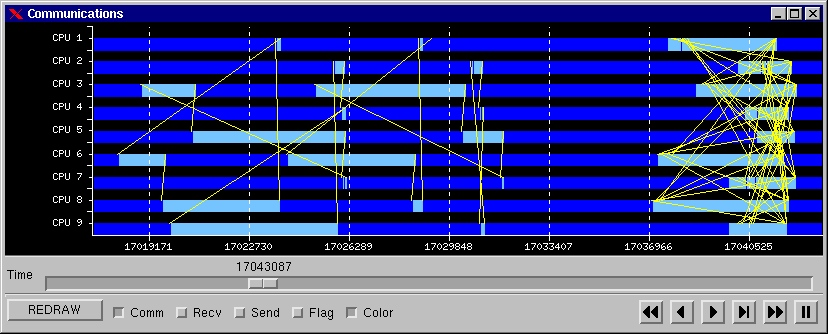
\includegraphics[width=0.7\textwidth]{paravertimeline}
    \end{figure}

    \pause

  \item[Statistics:] {\small (\emph{aka} \underline{Profile window})}
    Numerical analysis of the data
    \begin{figure}
      \hspace*{-0.5cm}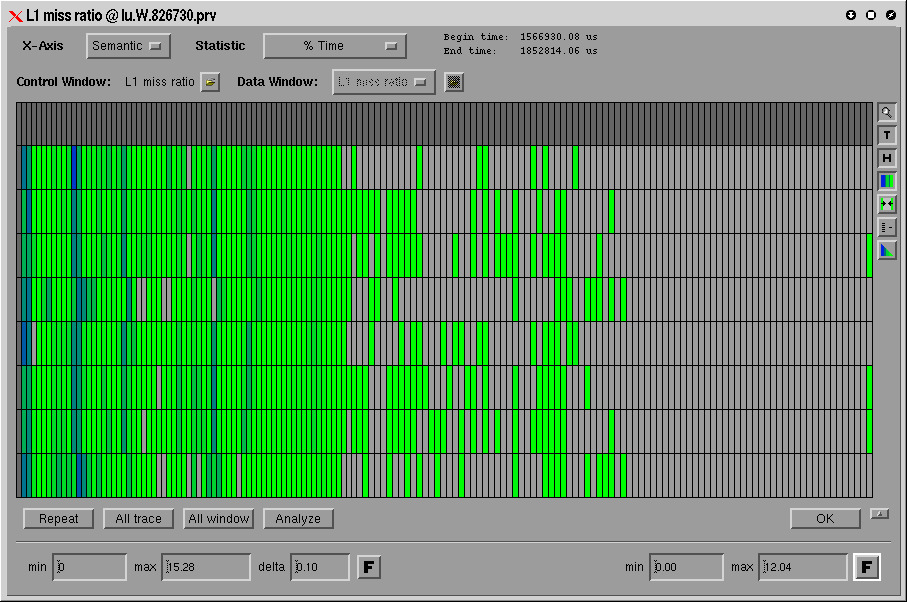
\includegraphics[width=0.4\textwidth]{paraverhistogram}
      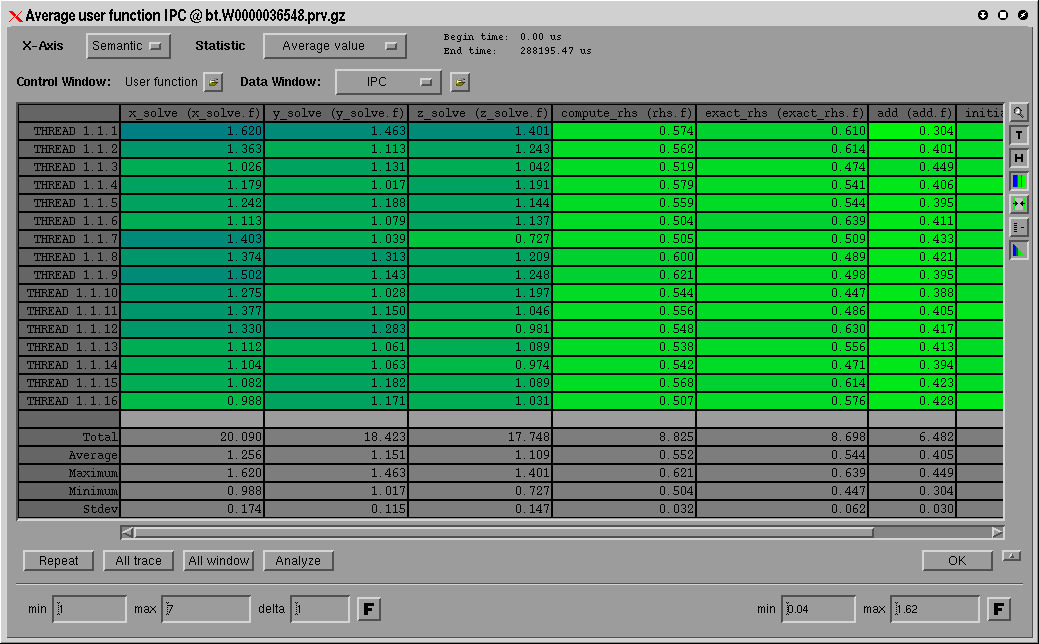
\includegraphics[width=0.43\textwidth]{paraverdata}
    \end{figure}
  \end{description}
}

% \subsection{Shared memory (OpenMP)}

% \frame{
% }

% \subsubsection{Load balancing optimization}

% \frame{
% }

% \subsubsection{Communication analysis and optimization}

% \frame{
% }

% \subsection{Distributed memory (MPI)}

% \frame{
% }

% \subsubsection{Load balancing optimization}

% \frame{
% }

% \subsubsection{Communication analysis and optimization}

% \frame{
% }

% \subsection{Hybrid parallel programming: shared + distributed Mem}

% \frame{
% }

% \subsubsection{Load balancing optimization}

% \frame{
% }

% \subsubsection{Communication analysis and optimization}

% \frame{
% }

\end{document}